In this chapter the results of the simulations performed in context of thesis are
presented. The aim of this computational analysis is to shed light on the entropic
effects which play a central role in the nanopiston's operating cycle. By extension the
thermodynamic transitions providing the free energy governing its operation are
simulated.

To study the entropic interactions between the DNA rotaxane and the nanopore an attempt
is made to isolate its effect using a specially engineered rotaxane variant. This other
class of rotaxane is called the mixed rotaxane, composing of a fraction of ds- and
ssDNA. Having laid the basis to understand the entrpoc contributions, next Then conformal
fluctuations of the nanopiston are simulated and analysed. Lastly an attempt is made to
simulate the thermodynamics transiditon of the dna piston cycle. forward flux sampling
entropic contributions.

\section{Mixed Rotaxane}

- explain what we study rotaxanes.
  here we study the mixed rotaxane fractions: ds100-ss0, ds90-ss10, ds80-ss20, ds70-ss30.

  Experimentally, the I-V measurements where  perfoperformed for these structures, by
  Bayoumi et al.

  explain what we see in the I-V measurements. -> blockage

- How we analyse the simulations.
  To understand and give meaning to the I-V curves we perform simulations of the mixed
  rotaxanes at 0 V.
  Track the reaction coordinate of the neutravidin protein located at the trans side. The
  reaction coordinate is defined as,
\begin{equation}
  X = \begin{cases}
        &Z_0 + |\textbf{r} - \textbf{r}_{cis}|, \hspace{0.5cm} \textit{if on cis-side}\\
        &Z, \hspace{2.5cm} \textit{if inside pore}\\
        &-|\textbf{r}|, \hspace{2.11cm} \textit{if on trans-side}
      \end{cases}
\end{equation}
Explain what we see: entropic force!



%% Zelf nog schrijven
% To highlight the crucial role of the entropic forces, we designed and studied four
% different rotaxanes, hereby referred to as mixed rotaxanes. These are an alternative
% version of rotaxane-ds, in which the toehold is removed, and the ssDNA connection strand
% varied in length. the total length of the rotaxane thread was fixed at 100 nt/bp, with
% the ss-DNA connection strand length varying from 0 nt to 40 nt and the ds DNA varying
% from 100 bp to 60 bp, in steps of 10 nt/bp
%
% We then performed I-V measurements in the range, see figure.
%
% The mixed rotaxane composed entirely of dsDNA yields an almost linear I-V plot in the
% measured voltage range indicating a constant obstruction of the nanopore. constant
% resistance of the nanopore.
%
% The rotaxane with a 10 nt ssDNA, however, has a rather different behavior. Observed
% blockage at high voltages in experiments.
%
% Longer strands we observe no blockage.
%
% Shed light on these experimental results we performed MD Simulations at zero bias, here
% the entropic contributions can be isolated.
%
% 1D diffusion
%
% We identify the z-axis with the symmetry axis of the pore and fix the origin of the
% coordinate system at the center of the trans-entry of the pore. The center of the cis
% entry is then located at $r_{cis} = (0, 0, z_{0})$ , with respect to the origin,
% where $z_0 = 14.3\ nm$ (see Figure S6). We define the reaction coordinate as follows
%
%
% The simulation data show that the peak gradually shifts towards negative values of $X$
% with increasing ssDNA length, suggesting that full pore blockage requires increasingly
% stronger electrophoretic force.

% To gain some insight on these entropic forces, we performed computer simulations of the
% rotaxane/ClyA complex in absence of an applied potential ($\Delta V = 0$)
%
% We identify the z-axis with the symmetry axis of the pore and fix the origin of the
% coordinate system at the center of the trans-entry of the pore. The center of the cis
% entry is then located at $r_{cis} = (0, 0, z_{0})$ , with respect to the origin,
% where $z_0 = 14.3\ nm$ (see Figure S6). We define the reaction coordinate as follows








\begin{figure}[ht]

  \begin{centering}
  \adjustbox{minipage=1.3em,valign=t}{\subcaption{}\label{sfig:testa}}%
  \begin{subfigure}[t]{\dimexpr.29\linewidth-1.3em\relax}
  \centering
  \vspace{0.6cm}
  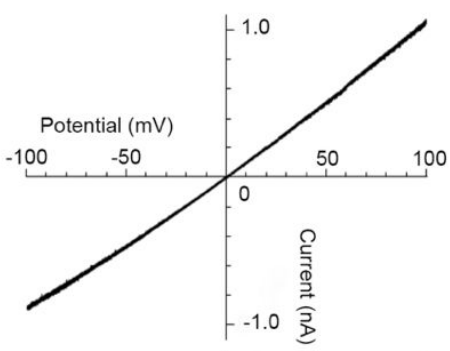
\includegraphics[width=1\linewidth,valign=t]{Figures/IV-100.png}
  \end{subfigure}%
  \adjustbox{minipage=1.3em,valign=t}{\subcaption{}\label{sfig:testb}}%
  \begin{subfigure}[t]{\dimexpr.5\linewidth-1.3em\relax}
  \centering
  \vspace{-0.1cm}
  \includegraphics[width=\linewidth,valign=t]{Figures/MR-100.png}
  \end{subfigure}%
  \adjustbox{minipage=1.3em,valign=t}{\subcaption{}\label{sfig:testc}}%
  \begin{subfigure}[t]{\dimexpr.21\linewidth-1.3em\relax}
  \centering
  \vspace{0.3cm}
  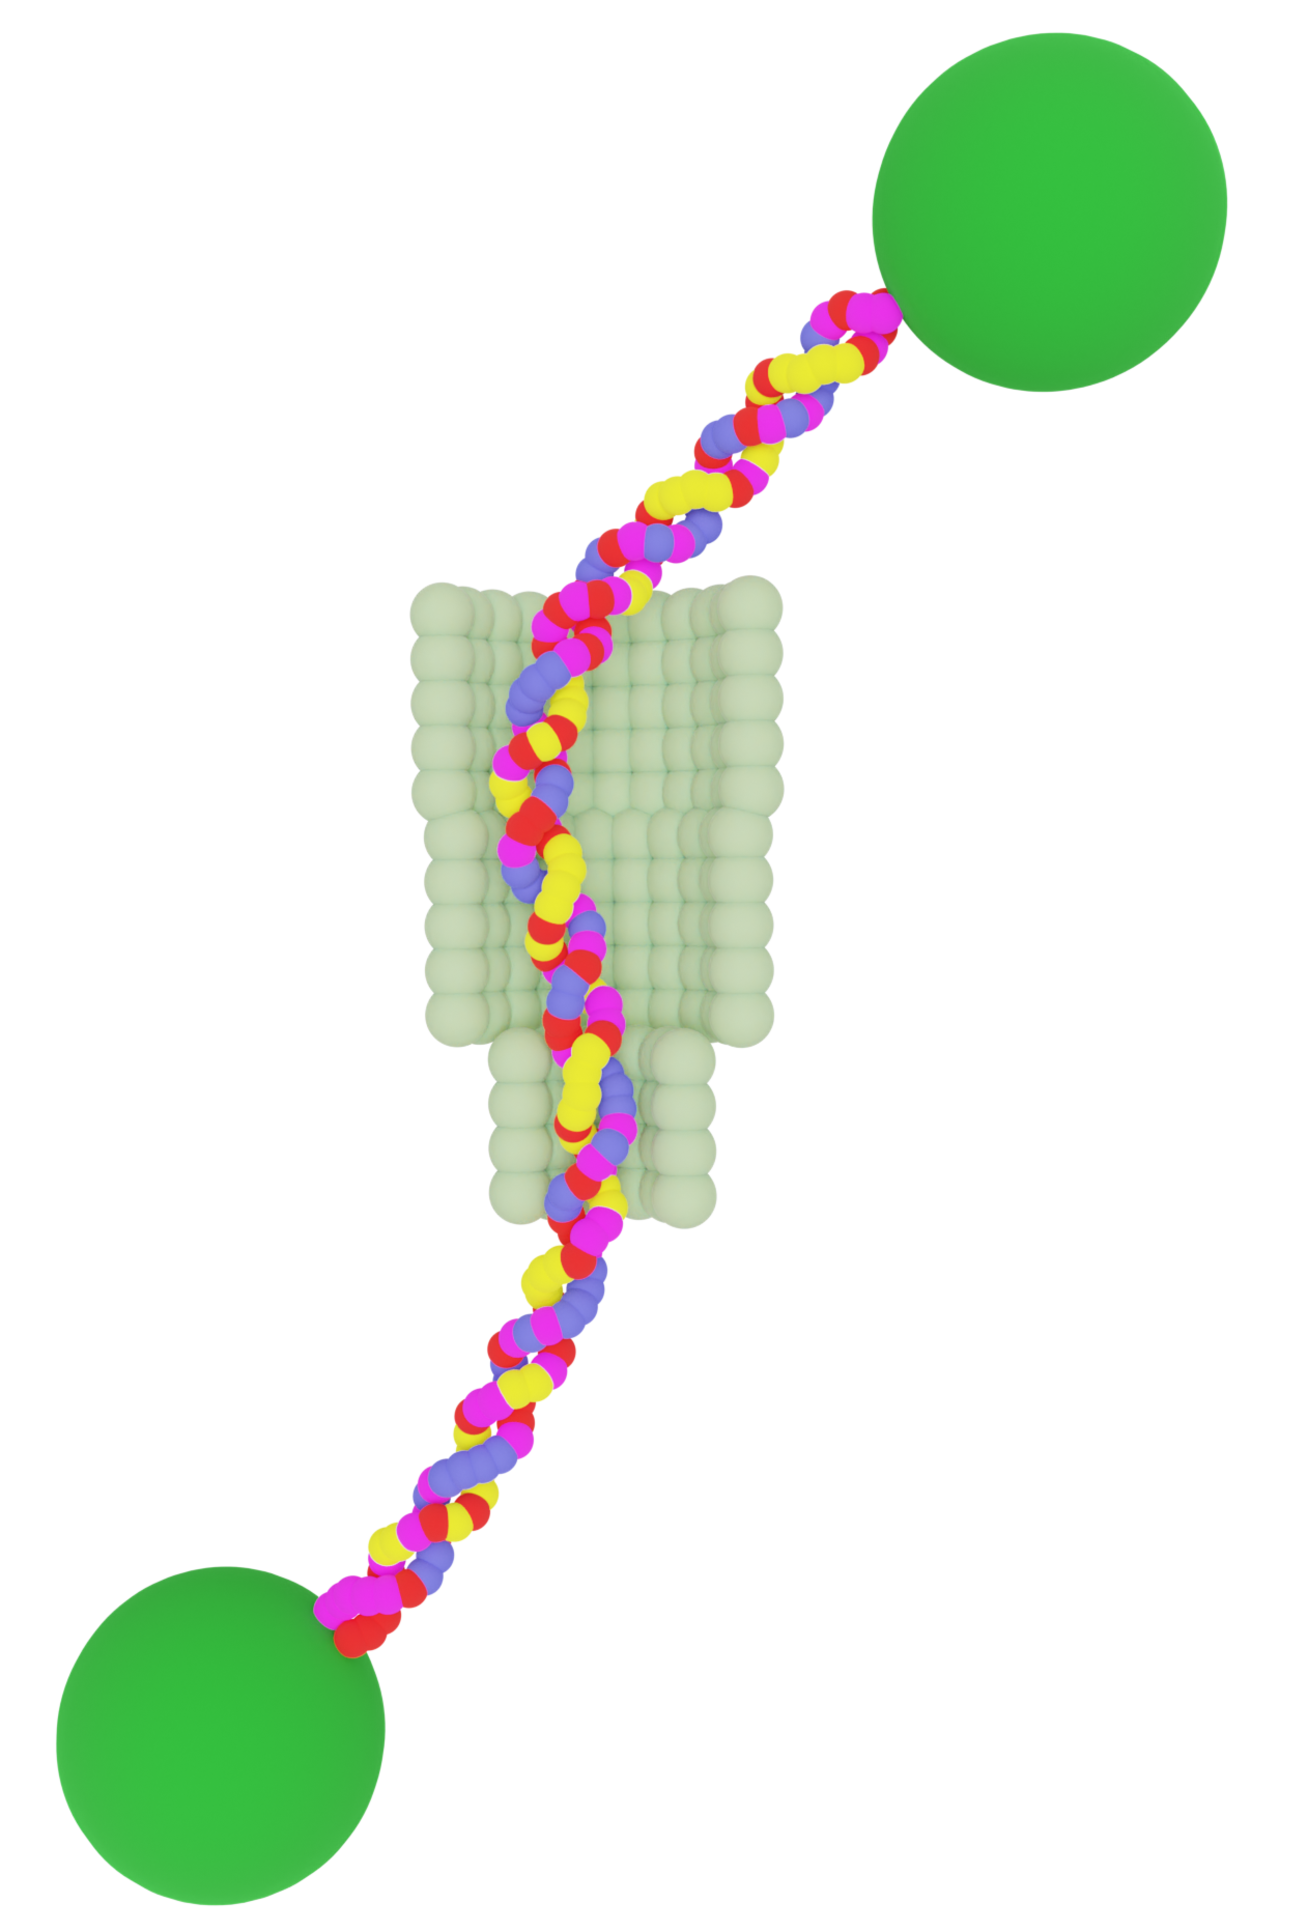
\includegraphics[width=\linewidth,valign=t]{Figures/Rotaxane-100.png}
  \end{subfigure}
  \label{fig:test}
  \end{centering}

  \vspace{0.01cm}

  \begin{centering}
  \adjustbox{minipage=1.3em,valign=t}{}%
  \hspace{.35cm}
  \begin{subfigure}[t]{\dimexpr.3\linewidth-1.3em\relax}
  \centering
  \vspace{0.2cm}
  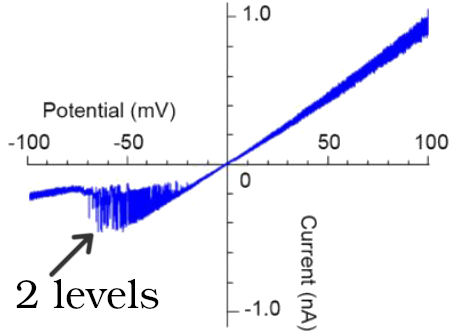
\includegraphics[width=\linewidth,valign=t]{Figures/IV-90.png}
  \end{subfigure}%
  \adjustbox{minipage=1.3em,valign=t}{}%
  \hspace{.25cm}
  \begin{subfigure}[t]{\dimexpr.5\linewidth-1.3em\relax}
  \centering
  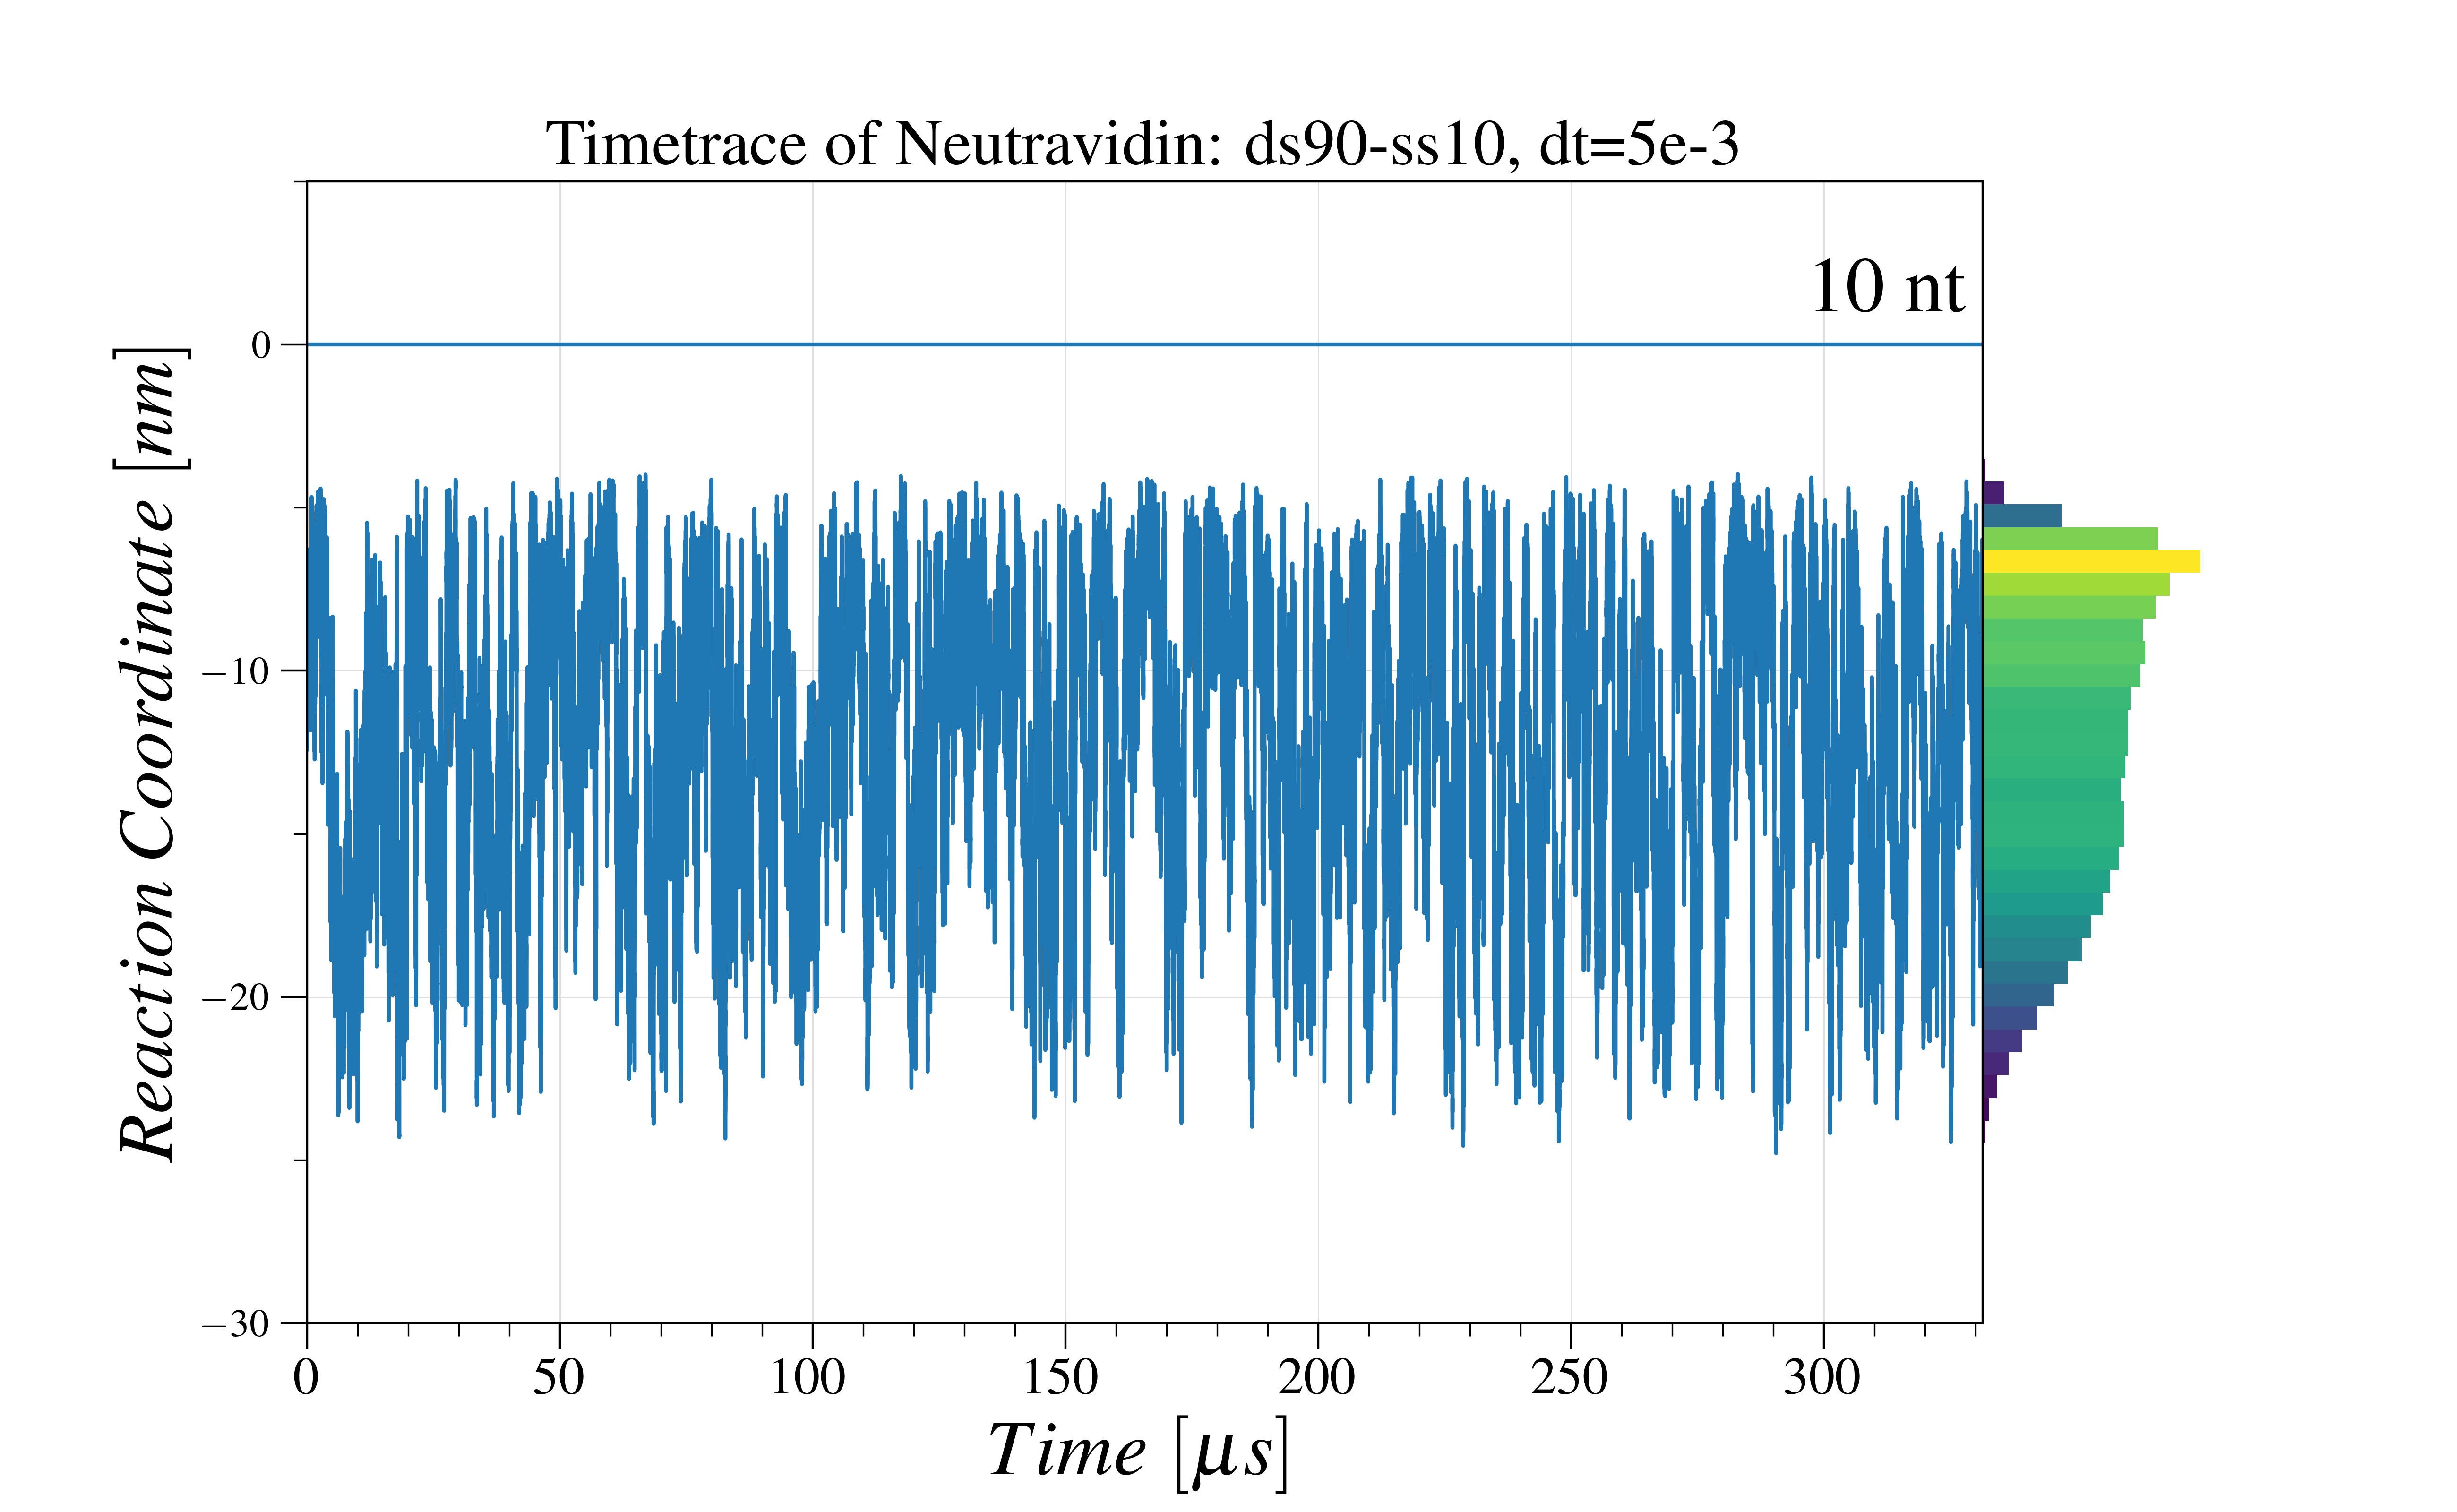
\includegraphics[width=\linewidth,valign=t]{Figures/MR-90.png}
  \end{subfigure}%
  \adjustbox{minipage=1.3em,valign=t}{}%
  \hspace{.3cm}
  \begin{subfigure}[t]{\dimexpr.21\linewidth-1.3em\relax}
  \centering
  \vspace{-0.5cm}
  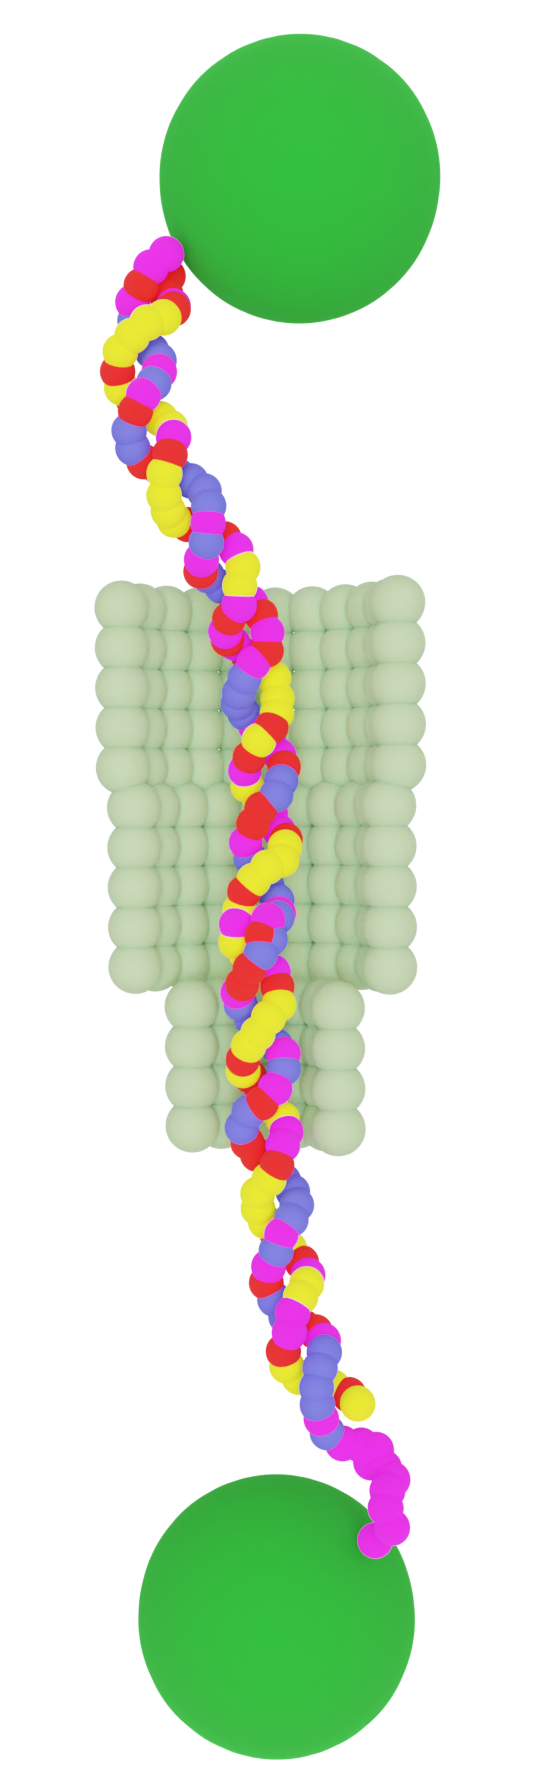
\includegraphics[width=.5\linewidth,valign=t]{Figures/Rotaxane-90.png}
  \end{subfigure}
  \label{fig:test}
  \end{centering}

  \vspace{.01cm}

  \begin{centering}
  \adjustbox{minipage=1.3em,valign=t}{}%
  \begin{subfigure}[t]{\dimexpr.3\linewidth-1.3em\relax}
  \centering
  \vspace{0.2cm}
  \hbox{\hspace{0.35cm}
  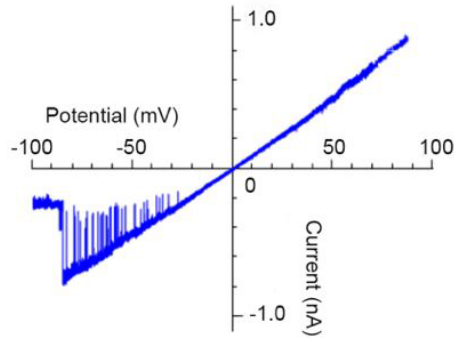
\includegraphics[width=1\linewidth,valign=t]{Figures/IV-80.png}}
  \end{subfigure}%
  \adjustbox{minipage=1.3em,valign=t}{}%
  \hspace{-0.5cm}
  \begin{subfigure}[t]{\dimexpr.5\linewidth-1.3em\relax}
  \centering
  \hbox{\hspace{0.51cm}
  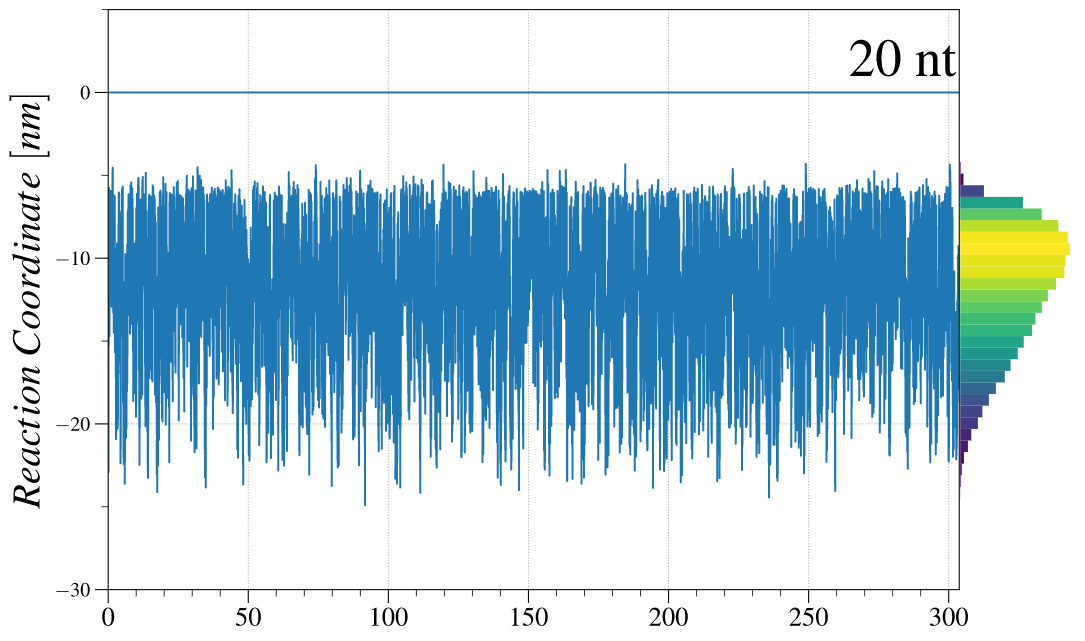
\includegraphics[width=\linewidth,valign=t]{Figures/MR-80.png}}
  \end{subfigure}%
  \adjustbox{minipage=1.3em,valign=t}{}%
  \hspace{.5cm}
  \begin{subfigure}[t]{\dimexpr.21\linewidth-1.3em\relax}
  \centering
  \vspace{-0.5cm}
  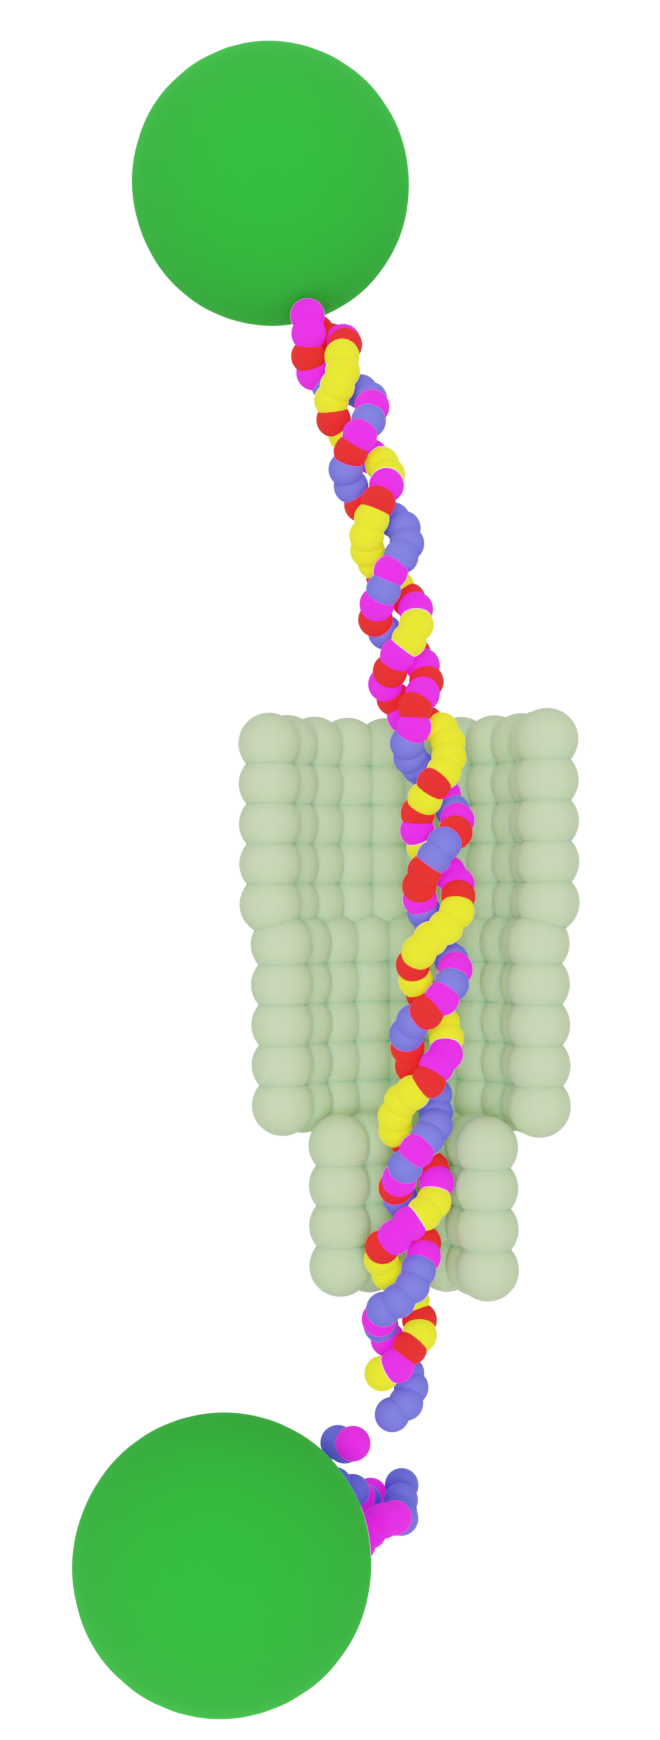
\includegraphics[width=.6\linewidth,valign=t]{Figures/Rotaxane-80.png}
  \end{subfigure}
  \label{fig:test}
  \end{centering}

  \vspace{.01cm}

  \begin{centering}
  \adjustbox{minipage=1.3em,valign=t}{}%
  \begin{subfigure}[t]{\dimexpr.3\linewidth-1.3em\relax}
  \centering
  \vspace{0.2cm}
  \hbox{\hspace{0.4cm}
  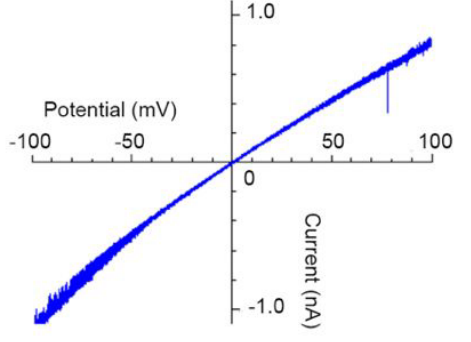
\includegraphics[width=\linewidth,valign=t]{Figures/IV-70.png}}
  \end{subfigure}%
  \adjustbox{minipage=1.3em,valign=t}{}%
  \begin{subfigure}[t]{\dimexpr.5\linewidth-1.3em\relax}
  \centering
  \hbox{\hspace{0.1cm}
  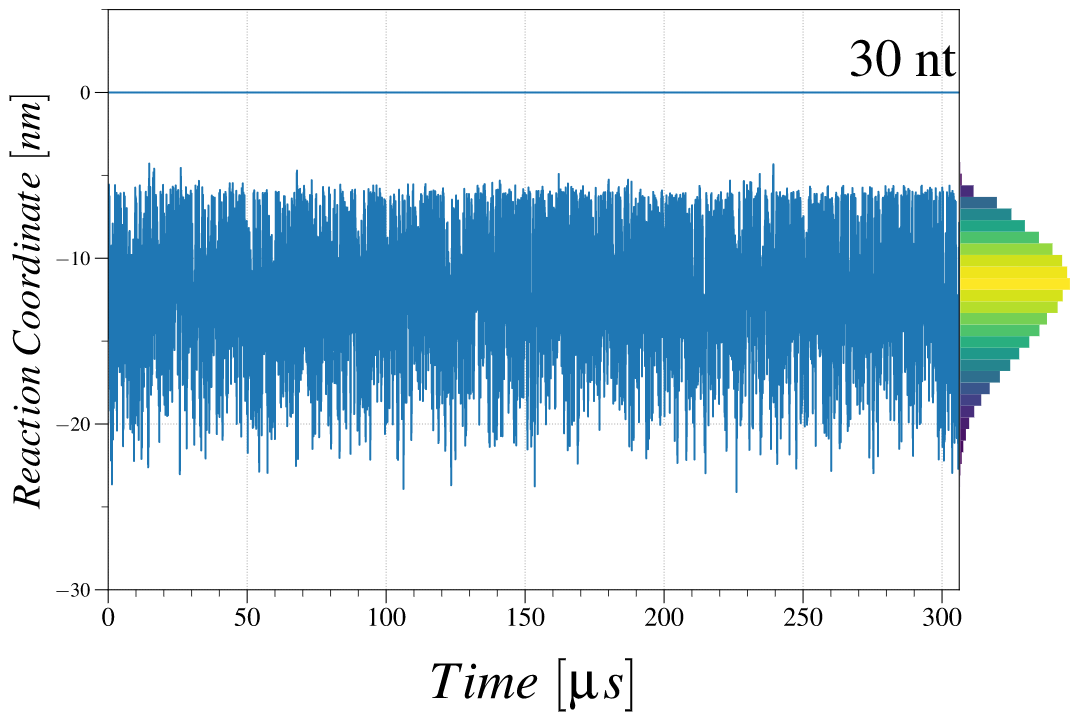
\includegraphics[width=\linewidth,valign=t]{Figures/MR-70.png}}
  \end{subfigure}%
  \adjustbox{minipage=1.3em,valign=t}{}%
  \hspace{0.5cm}
  \begin{subfigure}[t]{\dimexpr.21\linewidth-1.3em\relax}
  \centering
  \vspace{-0.5cm}
  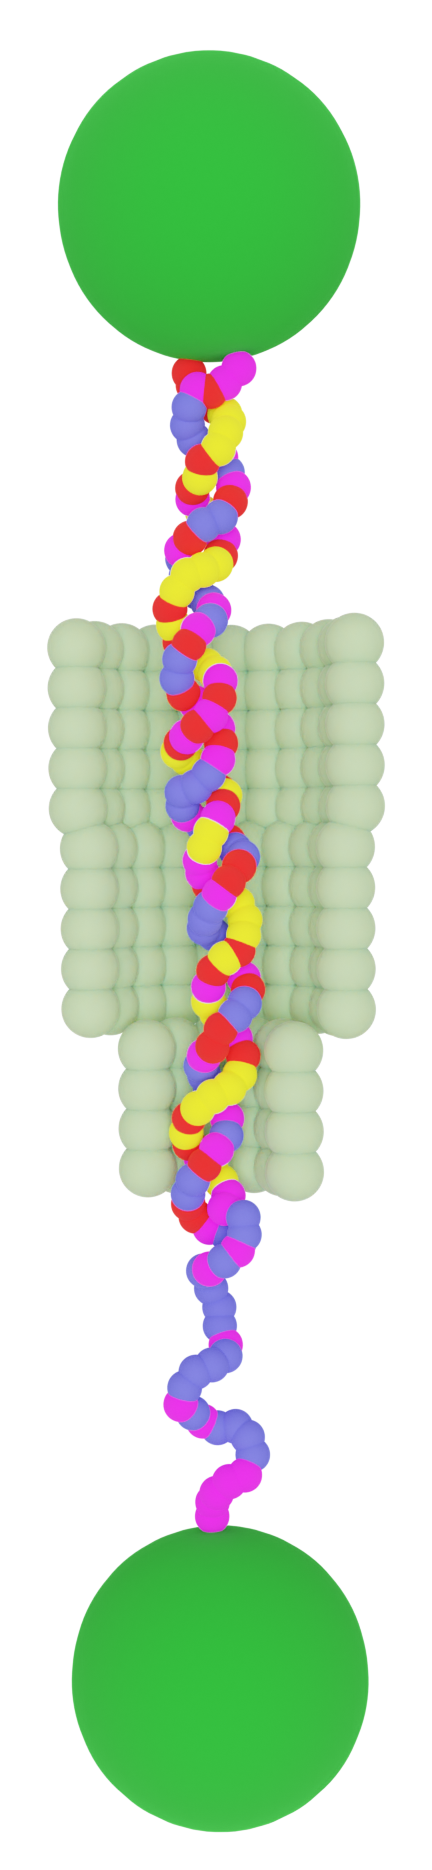
\includegraphics[width=.4\linewidth,valign=t]{Figures/Rotaxane-70.png}
  \end{subfigure}
  \label{fig:test}
  \end{centering}
  \caption{This is a figure.}

\end{figure}



\begin{figure}
\begin{center}
  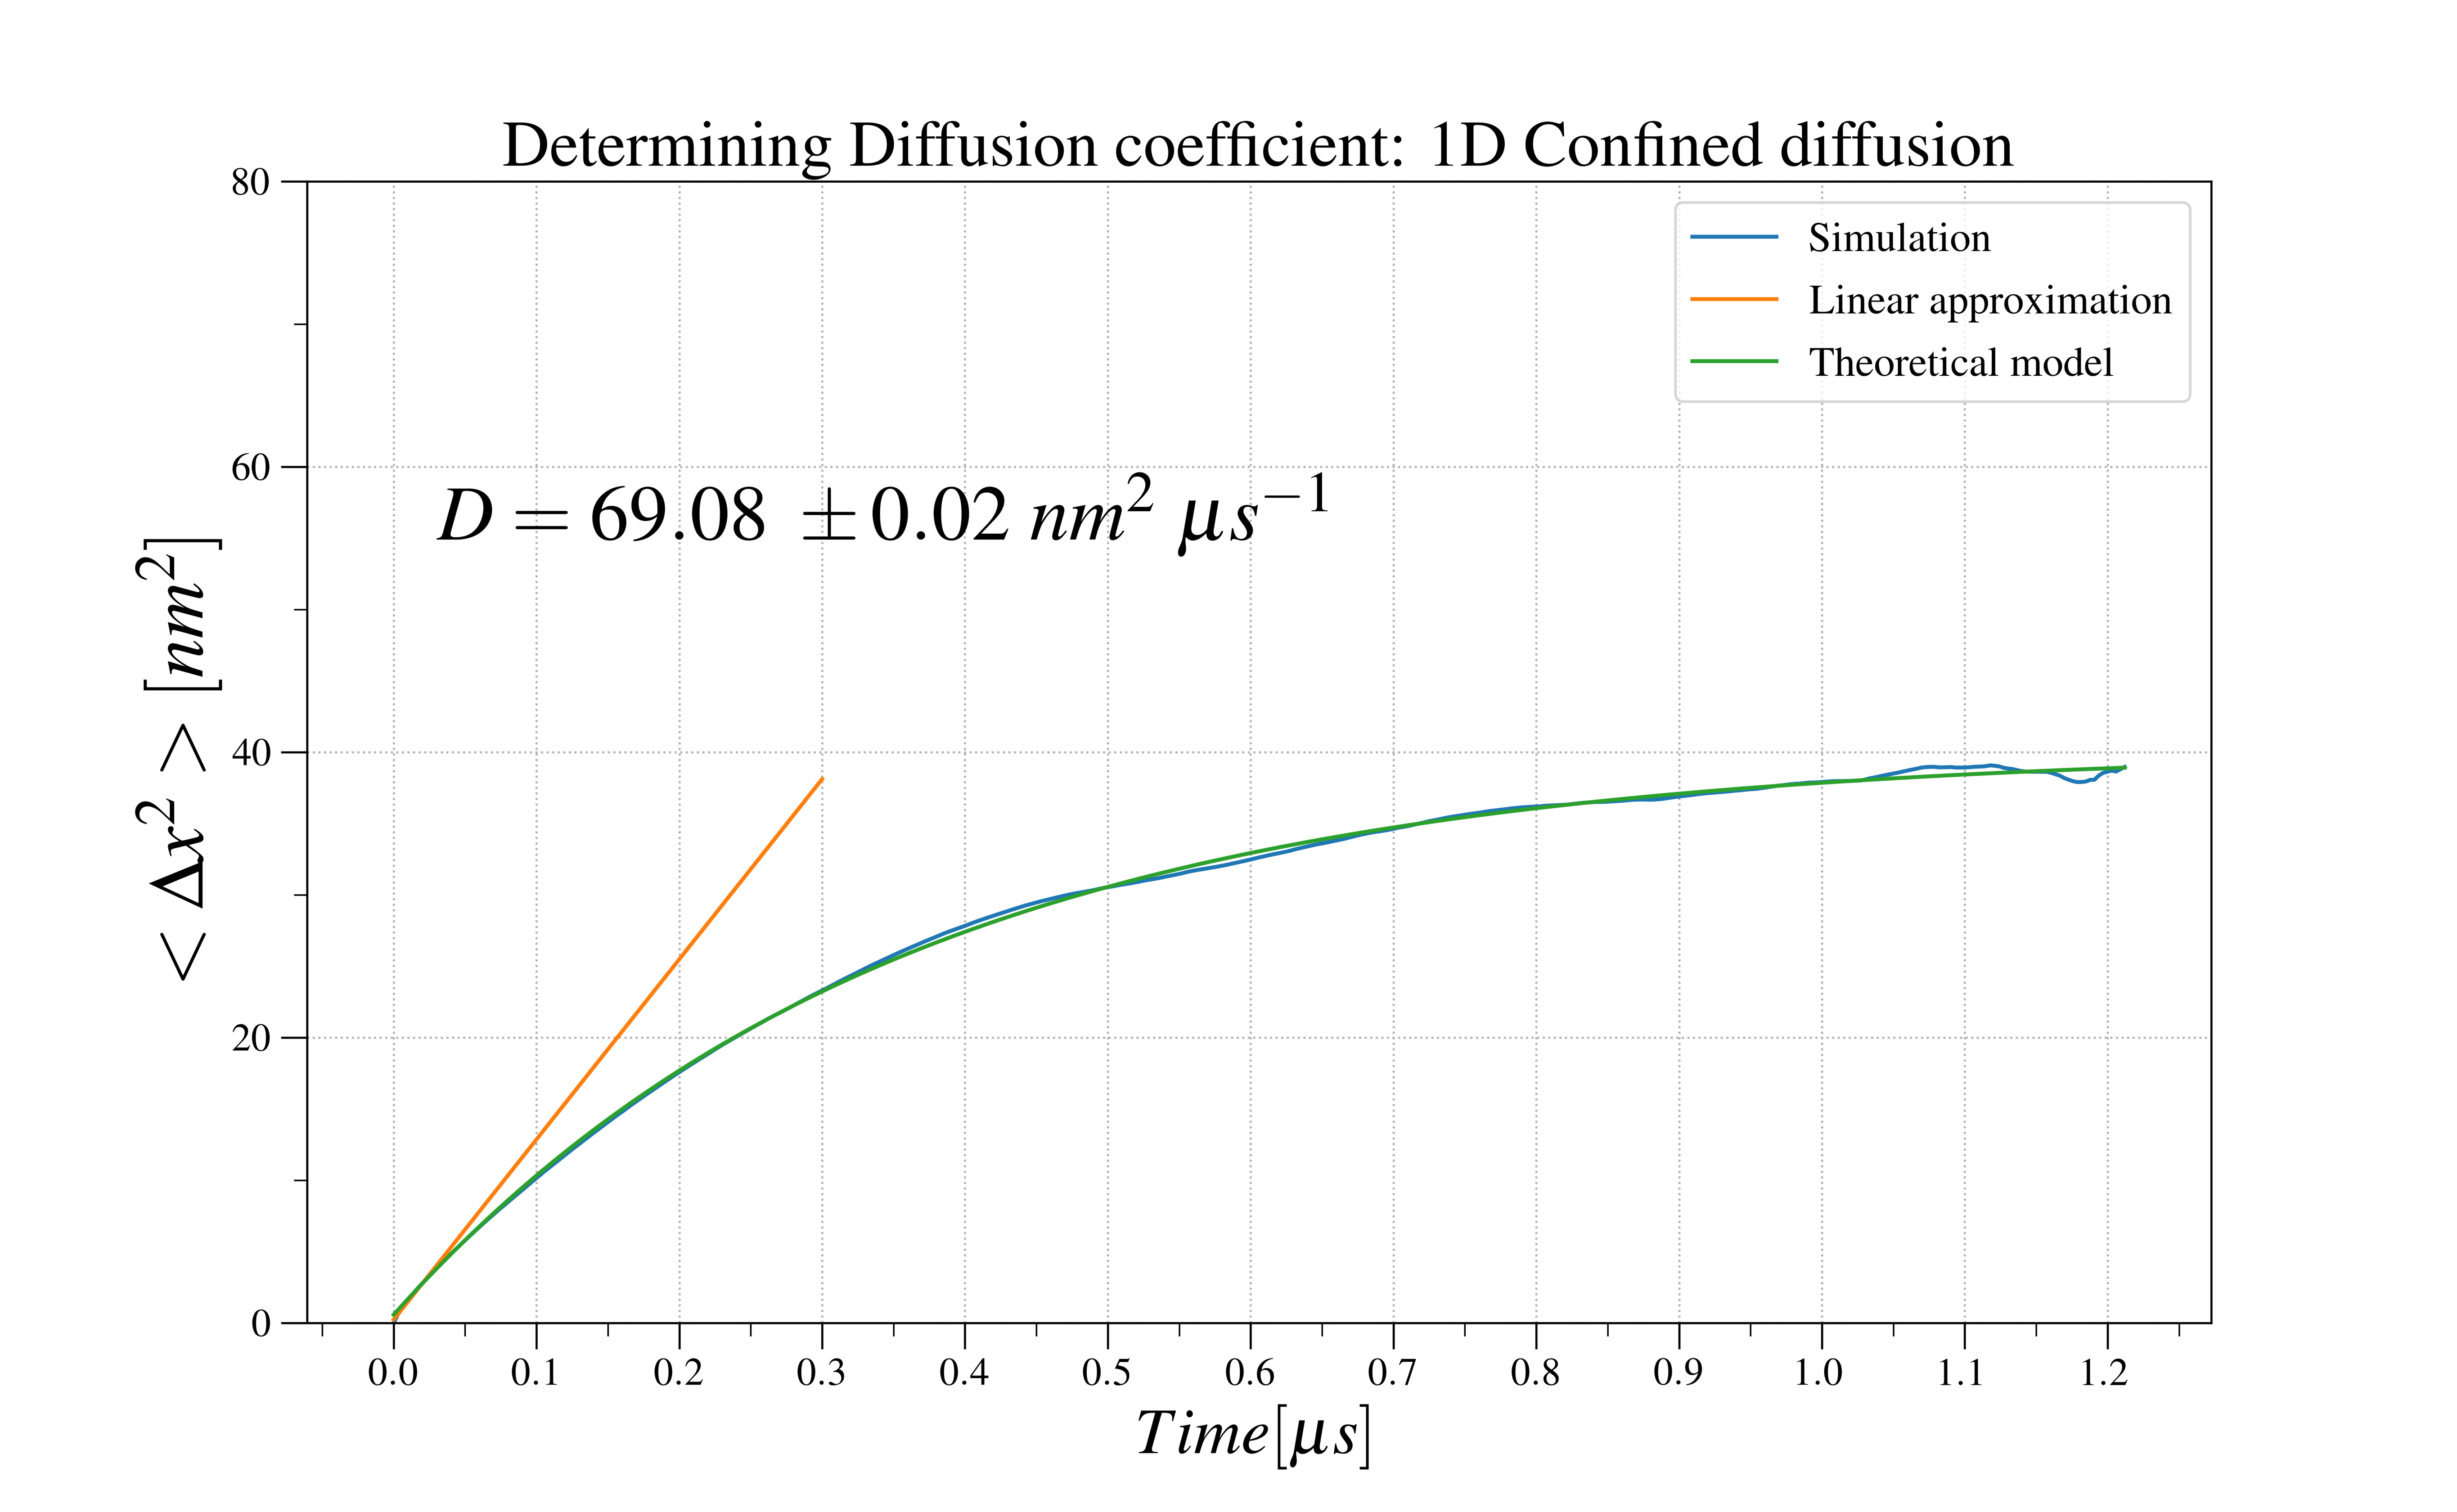
\includegraphics[width=0.90\textwidth]{Figures/MR-100-diff.png}
  \caption{write caption}
\end{center}
\end{figure}
